\documentclass[11pt,a4paper]{article}

\usepackage[margin=1in]{geometry}
\usepackage[T1]{fontenc}
\usepackage{lmodern}
\usepackage{amsmath,amssymb}
\usepackage{graphicx}
\usepackage{booktabs}
\usepackage{array}
\usepackage[font=small,labelfont=bf]{caption}
\usepackage{enumitem}
\usepackage{placeins}
\usepackage[hidelinks]{hyperref}

% Figures are read directly from the output folders of the code
\graphicspath{{../Task-1/results/}{../Task-5/results/}}

\setlist{itemsep=2pt,topsep=4pt}
\setlength{\parindent}{0pt}
\setlength{\parskip}{5pt}

% Notation
\newcommand{\Ncp}{N_{\mathrm{cp}}}
\newcommand{\SNR}{\mathrm{SNR}}
\newcommand{\E}{\mathbb{E}}
\newcommand{\yt}{\tilde{y}}
\newcommand{\dt}{\tilde{d}}
\newcommand{\deq}{\hat{\tilde{d}}}
\newcommand{\wt}{\tilde{w}}

\begin{document}

\begin{center}
  {\LARGE EC5.407 Wireless Communications - Assignment 3}\\[6pt]
  {\large Design of an OFDM Link for a 5G NR-like Downlink}\\[12pt]
  {\large Ande Karthik \qquad 2023102009}\\[6pt]
  \textbf{Code:} \texttt{\url{https://github.com/KarthiK-Ande-22/Wireless-Communication-Assignment-3}}
\end{center}

\vspace{6pt}

% =====================================================================
\section{Simulation set-up}
% =====================================================================

\subsection{System model and conventions}

The link follows Section 2 of the assignment. One slot has 14 OFDM symbols,
$i = 0, \ldots, 13$, and every OFDM symbol has $N = 512$ subcarriers,
$k = 0, \ldots, N-1$. Each resource element carries one 4-QAM symbol.
Table~\ref{tab:parameters} lists the parameters.

\begin{table}[!htb]
  \centering
  \caption{System parameters (Table 2 of the assignment) and the values derived from them.}
  \label{tab:parameters}
  \begin{tabular}{ll}
    \toprule
    Parameter & Value \\
    \midrule
    Bandwidth = sampling rate $W$         & 15.36 MHz, sample period $1/W = 65.1$ ns \\
    Number of subcarriers (DFT size) $N$  & 512 \\
    Subcarrier spacing $\Delta f = W/N$   & 30 kHz \\
    OFDM symbol duration without CP $N/W$ & 33.33 $\mu$s \\
    OFDM symbols per slot                 & 14 \\
    Data symbols per slot                 & $14 \times 512 = 7168$ \\
    Modulation                            & 4-QAM, $\E|s[n]|^2 = 1$ \\
    SNR                                   & 30 dB (noise power $1/\SNR = 10^{-3}$) \\
    CP length $\Ncp$ (Task 1)             & 4 (Scenario 1) and 75 samples (Scenario 2) \\
    \bottomrule
  \end{tabular}
\end{table}

\begin{itemize}
  \item \textbf{4-QAM:} the points $(\pm 1 \pm j)/\sqrt{2}$, the same function as in Assignment 2.
        Every point has $|s| = 1$, so the average energy is exactly 1.
  \item \textbf{Unitary DFT:} $F^H \dt = \sqrt{N}\,\texttt{ifft}(\dt)$ and $F y = \texttt{fft}(y)/\sqrt{N}$,
        as in Section 4 of the assignment. Because $F$ is unitary, every time sample has
        $\E|d_i[m]|^2 = 1$, so the transmitted signal has $\E|x[m]|^2 = 1$, and the noise keeps its
        variance after the DFT.
  \item \textbf{Channel:} $h[\ell] \sim \mathcal{CN}(0, \sigma_\ell^2)$ with $\sum_\ell \sigma_\ell^2 = 1$
        (Table 1 of the assignment). One realization per scenario, constant over the slot and known
        at the receiver. The frequency response is $H[k] = \texttt{fft}(h, N)$.
  \item \textbf{Noise:} $w[m] \sim \mathcal{CN}(0, 1/\SNR)$, with independent real and imaginary parts.
        Since the signal power is 1, the SNR is the SNR per data subcarrier.
  \item \textbf{Seeds:} each random block has its own generator, \texttt{np.random.default\_rng(seed)}:
        data 2026, channel 2027 (Scenario 1) and 2028 (Scenario 2), noise 2029. So the data and the
        channel are the same in every run of a scenario. In Task 5(d) only the CP changes.
\end{itemize}

\subsection{Code structure}

Each block of Fig.~2 and Fig.~3 of the assignment is its own function, and each task has its own
folder. The code is Python 3.12 with NumPy, SciPy (only \texttt{erfc}, for the $Q$-function) and
Matplotlib. Only \texttt{fft}, \texttt{ifft} and \texttt{convolve} are used from NumPy; no built-in
OFDM or 5G function is used.

\begin{table}[!htb]
  \centering
  \caption{Files of the code. Shared numbers (Tables 1 and 2 of the assignment, seeds) are in \texttt{parameters.py}.}
  \label{tab:code}
  \small
  \begin{tabular}{>{\raggedright\arraybackslash}p{4.7cm}>{\raggedright\arraybackslash}p{10.0cm}}
    \toprule
    File & What it does \\
    \midrule
    \texttt{Task-1/cp\_design.py}  & Task 1: CP length, rms delay spread, and the ISI + ICI power of a too short CP (Sec.~\ref{sec:task1}, App.~\ref{app:interference}). \\
    \texttt{Task-2/transmitter.py} & Task 2: \texttt{generate\_data}, \texttt{map\_to\_resource\_grid}, \texttt{ofdm\_modulate}, \texttt{add\_cyclic\_prefix} and \texttt{concatenate\_symbols}. \\
    \texttt{Task-3/channel.py}     & Task 3: \texttt{channel\_taps}, \texttt{frequency\_response}, \texttt{multipath\_channel}. \\
    \texttt{Task-4/receiver.py}    & Task 4: \texttt{split\_into\_blocks}, \texttt{remove\_cyclic\_prefix}, \texttt{ofdm\_demodulate}, \texttt{equalize}, \texttt{demap\_resource\_grid}; and \texttt{detect\_symbols} (Assignment 2 detector, only to count errors). \\
    \texttt{Task-5/main.py}        & Task 5: main script. \texttt{main.py -{}-scenario S [-{}-cp Ncp]} runs the link for one scenario and CP length, and makes all figures of Task 5 and a \texttt{summary.txt}. \\
    \texttt{Task-5/plots.py}       & The figures of Task 5. \\
    \texttt{Task-5/cp\_sweep.py}   & Extra: the link for every $\Ncp$ from 0 to 80 (Sec.~\ref{sec:sweep}). \\
    \bottomrule
  \end{tabular}
\end{table}

\textbf{Reproducing.} \texttt{bash run\_all.sh} runs all scripts in under a minute and reproduces every
figure and number of this report exactly. Every number quoted below is read from the
\texttt{results/} folders; the README lists all commands.

\subsection{Check of every block}

Running the files of Tasks 2--4 directly checks each block (\texttt{results/*\_check.txt}):

\begin{table}[!htb]
  \centering
  \caption{Checks of the blocks. Bottom: the noise-free loopback sends a whole slot through transmitter, channel and receiver with $1/\SNR = 0$.}
  \label{tab:checks}
  \small
  \begin{tabular}{lll}
    \toprule
    Block & Check & Result \\
    \midrule
    DFT matrix          & $\max|F F^H - I|$                                          & $4.4 \cdot 10^{-14}$ \\
    IDFT (Task 2c)      & $\max|\sqrt{N}\,\texttt{ifft}(\dt) - F^H \dt|$              & $2.8 \cdot 10^{-13}$ \\
    DFT (Task 4a)       & $\max|\texttt{fft}(y_c)/\sqrt{N} - F y_c|$                  & $4.8 \cdot 10^{-13}$ \\
    Grid mapping        & $\dt_i[k] = s[Ni + k]$ for all $i, k$                       & true \\
    Cyclic prefix       & $\max|\text{CP} - \text{last } \Ncp \text{ samples}|$        & 0 (exact copy) \\
    $H[k]$              & $\max|\texttt{fft}(h, N) - \sum_\ell h[\ell] e^{-j2\pi k\ell/N}|$ & $1.2 \cdot 10^{-15}$ (S1), $1.2 \cdot 10^{-14}$ (S2) \\
    Tap generator       & $\E|h[\ell]|^2$ over 20\,000 draws                           & equal to $\sigma_\ell^2$ within 1\% \\
    Convolution         & length of $y$                                                & $M + L - 1$ \\
    Noise               & measured variance $\times \SNR$                               & 0.996 \\
    \bottomrule
  \end{tabular}

  \vspace{8pt}
  \begin{tabular}{llcc}
    \toprule
    Noise-free loopback & CP length & $\max|\yt_i[k] - H[k]\dt_i[k]|$ & $\max|\hat{s}[n] - s[n]|$ \\
    \midrule
    Scenario 1 & $\Ncp = 4 = L - 1$  & $1.0 \cdot 10^{-15}$ & $1.4 \cdot 10^{-15}$ \\
               & $\Ncp = 3$          & $1.2 \cdot 10^{-2}$  & $2.5 \cdot 10^{-2}$ \\
    Scenario 2 & $\Ncp = 75 = L - 1$ & $1.4 \cdot 10^{-15}$ & $6.7 \cdot 10^{-15}$ \\
               & $\Ncp = 74$         & $5.0 \cdot 10^{-3}$  & $1.0 \cdot 10^{-1}$ \\
    \bottomrule
  \end{tabular}
\end{table}

The loopback checks the CP condition of Task 1 directly: with $\Ncp = L - 1$ the receiver gets
the data back exactly (up to rounding errors), and with a CP only one sample shorter it does not.

% =====================================================================
\section{Task 1 --- CP length}
\label{sec:task1}
% =====================================================================

\subsection{Condition for no ISI and no ICI}

After removing the CP, the receiver keeps the samples $m = 0, \ldots, N-1$ of block $i$:
\begin{equation}
  y_{c,i}[m] = \sum_{\ell=0}^{L-1} h[\ell]\, x\big[i(N+\Ncp) + \Ncp + m - \ell\big] + w_{c,i}[m].
  \label{eq:window}
\end{equation}
Tap $\ell$ reads the transmitted sample at position $\Ncp + m - \ell$ inside block $i$.
\begin{itemize}
  \item If $\ell \le \Ncp$, this position is inside block $i$ for every $m \ge 0$. There $x_i$ holds
        $d_i[(m - \ell) \bmod N]$: a sample of $d_i$ itself ($m \ge \ell$) or its copy in the CP ($m < \ell$).
  \item If $\ell > \Ncp$, the first $\ell - \Ncp$ samples ($m < \ell - \Ncp$) read block $i-1$:
        the tap brings in the previous OFDM symbol.
\end{itemize}
So, if every non-zero tap has $\ell \le \Ncp$, the window holds a \emph{circular} convolution,
\begin{equation}
  y_{c,i}[m] = \sum_{\ell} h[\ell]\, d_i[(m - \ell) \bmod N] + w_{c,i}[m],
\end{equation}
and the unitary DFT turns it into a product on every subcarrier:
\begin{equation}
  \yt_i[k] = H[k]\, \dt_i[k] + \wt_i[k], \qquad \wt_i[k] \sim \mathcal{CN}(0, 1/\SNR).
  \label{eq:flat}
\end{equation}
Nothing of symbol $i-1$ is left (no ISI), and subcarrier $k$ depends only on $\dt_i[k]$ (no ICI).
The condition is
\begin{equation}
  \Ncp \ge L - 1, \qquad L - 1 = \text{delay of the last non-zero tap}.
  \label{eq:condition}
\end{equation}

\subsection{Design}

I choose the shortest CP that meets \eqref{eq:condition}, $\Ncp = L - 1$ (Table~\ref{tab:cp}).

\begin{table}[!htb]
  \centering
  \caption{CP design (\texttt{Task-1/results/cp\_design.txt}). The coherence bandwidth uses the rule of thumb $B_c \approx 1/(5\tau_{\mathrm{rms}})$.}
  \label{tab:cp}
  \begin{tabular}{lcc}
    \toprule
    & Scenario 1 & Scenario 2 \\
    \midrule
    Last non-zero tap $L - 1$                    & 4 samples          & 75 samples \\
    Maximum delay $(L-1)/W$                      & 0.260 $\mu$s       & 4.883 $\mu$s \\
    rms delay spread $\tau_{\mathrm{rms}}$       & 1.05 samples = 68 ns & 11.48 samples = 747 ns \\
    Coherence bandwidth $B_c$                    & 2.93 MHz $\approx$ 98 subcarriers & 0.27 MHz $\approx$ 9 subcarriers \\
    \midrule
    \textbf{CP length $\Ncp$ (samples)}          & \textbf{4}         & \textbf{75} \\
    \textbf{CP length $\Ncp/W$ ($\mu$s)}         & \textbf{0.260}     & \textbf{4.883} \\
    \textbf{CP overhead $\Ncp/(N + \Ncp)$}       & \textbf{0.78\%}    & \textbf{12.78\%} \\
    \midrule
    OFDM symbol with CP, $N + \Ncp$              & 516 samples = 33.59 $\mu$s & 587 samples = 38.22 $\mu$s \\
    Slot, $M = 14(N + \Ncp)$                     & 7224 samples = 470.3 $\mu$s & 8218 samples = 535.0 $\mu$s \\
    \bottomrule
  \end{tabular}
\end{table}

\textbf{Why not shorter.} A tap beyond the CP causes ISI and ICI. Appendix~\ref{app:interference}
shows that their average power per subcarrier is
\begin{equation}
  P_{\mathrm{int}} = \frac{2}{N} \sum_{\ell} \sigma_\ell^2 \max(\ell - \Ncp, 0).
  \label{eq:pint}
\end{equation}
Fig.~\ref{fig:interference} plots it against $\Ncp$.
\begin{itemize}
  \item Each tap counts with its \emph{excess delay} $\ell - \Ncp$, so weak but late taps still matter.
        In Scenario 2 the two last taps carry only 0.9\% and 0.4\% of the power, but every tap
        ($\sigma_\ell^2 \ge 0.004$) is stronger than the noise ($1/\SNR = 0.001$).
  \item Even a softer rule, ``interference at least 10 dB below the noise'', needs $\Ncp \ge 4$ in
        Scenario 1 and $\Ncp \ge 69$ in Scenario 2. Going from 69 to 75 costs only 6 samples
        (11.9\% instead of 12.8\% overhead) and removes the interference completely, so I keep
        $\Ncp = L - 1$.
\end{itemize}

\textbf{Why not longer.} In this model (perfect timing, exact channel) a CP longer than $L-1$ brings
nothing. It only costs time and energy: the CP takes $\Ncp/(N + \Ncp)$ of the slot and of the
transmitted energy, and the receiver throws it away. This is 0.78\% (0.03 dB) in Scenario 1 and
12.78\% (0.59 dB) in Scenario 2. A real system would add a few samples of margin for timing errors
and filter tails.

\textbf{Comparison with 5G NR.} With 30 kHz spacing, NR uses a normal CP of 2.34 $\mu$s, which is
36 samples at this sampling rate (6.6\% overhead). Scenario 1 (0.26 $\mu$s) fits easily. Scenario 2
needs about twice as much: with a 36-sample CP its taps at 55 and 75 would leave an average
interference of $-28.9$ dB, as large as the noise (Fig.~\ref{fig:interference}).

\begin{figure}[!htb]
  \centering
  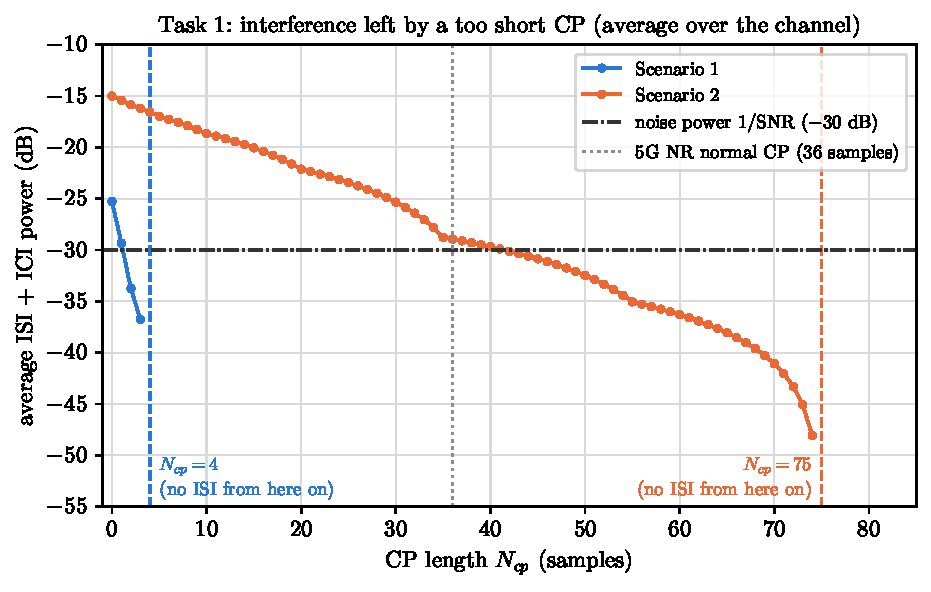
\includegraphics[width=0.85\textwidth]{interference_vs_cp.pdf}
  \caption{Task 1, both scenarios: average ISI + ICI power per subcarrier \eqref{eq:pint} against
    the CP length (average over the channel). Dash-dot: noise power $1/\SNR$. Dashed: the chosen
    $\Ncp = L - 1$ (4 and 75), from where the interference is exactly zero. Dotted: the 5G NR normal
    CP of 36 samples. \textbf{Every sample of CP below $L-1$ adds interference; in Scenario 2 it stays
    above the noise up to $\Ncp = 41$.}}
  \label{fig:interference}
\end{figure}

\FloatBarrier
% =====================================================================
\section{Task 2 --- Transmitter}
% =====================================================================

The transmitter (\texttt{Task-2/transmitter.py}) has one function per block of Fig.~2 of the assignment.
\begin{enumerate}[label=(\alph*)]
  \item \textbf{Data generation} (\texttt{generate\_data}): 7168 indices drawn uniformly from
        $\{0, 1, 2, 3\}$ select the 4-QAM points. Since $|s[n]| = 1$, the average energy is exactly 1.
  \item \textbf{Resource grid mapping} (\texttt{map\_to\_resource\_grid}): $s$ is cut into 14 rows of
        512 symbols, and the result is transposed. Column $i$ is $\dt_i$, with $\dt_i[k] = s[Ni + k]$.
  \item \textbf{OFDM modulation}: \texttt{ofdm\_modulate} computes $D = F^H \tilde{D} = \sqrt{N}\,
        \texttt{ifft}(\tilde{D})$ column by column, for all 14 symbols at once.
        \texttt{add\_cyclic\_prefix} puts the last $\Ncp$ rows on top, and
        \texttt{concatenate\_symbols} reads the $(N + \Ncp) \times 14$ array column after column.
        The result $x$ has $M = 14(N + \Ncp)$ samples: 7224 in Scenario 1 and 8218 in Scenario 2.
\end{enumerate}
\textbf{Energy.} By Parseval, $\|d_i\|^2 = \|\dt_i\|^2 = N$ exactly, because $|s[n]| = 1$. Without a
CP the average power of $x$ would be exactly 1. The CP repeats $\Ncp$ random samples, so the
measured average power is 1.0000 (Scenario 1, 4 CP samples) and 0.9946 (Scenario 2, 75 CP samples).

% =====================================================================
\section{Task 3 --- Channel}
% =====================================================================

The channel is in \texttt{Task-3/channel.py}.
\begin{itemize}
  \item \texttt{channel\_taps}: a vector of length $L$ = largest delay + 1 (5 in Scenario 1, 76 in
        Scenario 2). It is zero except at the taps of Table 1 of the assignment, where
        $h[\ell] = \sigma_\ell (a + jb)/\sqrt{2}$ with $a, b \sim \mathcal{N}(0, 1)$.
  \item \texttt{multipath\_channel}: $y = \texttt{convolve}(x, h) + w$, of length $M + L - 1$
        (7228 and 8293). The last $L - 1$ samples are the tail of the last OFDM symbol and are not used.
  \item \texttt{frequency\_response}: $H[k] = \texttt{fft}(h, N)$, used by the equalizer.
\end{itemize}
Table~\ref{tab:taps} gives the realization of each scenario.

\begin{table}[!htb]
  \centering
  \caption{Channel realizations (\texttt{Task-3/results/channel\_check.txt}), channel seed 2027 (Scenario 1) and 2028 (Scenario 2). All other taps are zero.}
  \label{tab:taps}
  \small
  \begin{tabular}[t]{rccc}
    \multicolumn{4}{c}{Scenario 1} \\
    \toprule
    $\ell$ & $\sigma_\ell^2$ & $h[\ell]$ & $|h[\ell]|^2$ \\
    \midrule
    0 & 0.539 & $+0.0576 - 0.0435j$ & 0.0052 \\
    1 & 0.271 & $-0.2960 - 0.7922j$ & 0.7152 \\
    2 & 0.136 & $+0.3160 - 0.1257j$ & 0.1157 \\
    4 & 0.054 & $-0.0320 - 0.1451j$ & 0.0221 \\
    \midrule
    \multicolumn{3}{l}{$\|h\|^2$} & 0.8582 \\
    \bottomrule
  \end{tabular}
  \qquad
  \begin{tabular}[t]{rccc}
    \multicolumn{4}{c}{Scenario 2} \\
    \toprule
    $\ell$ & $\sigma_\ell^2$ & $h[\ell]$ & $|h[\ell]|^2$ \\
    \midrule
     0 & 0.277 & $-0.0892 + 0.4362j$ & 0.1983 \\
     2 & 0.219 & $-0.4915 - 0.5895j$ & 0.5890 \\
     5 & 0.174 & $-0.2786 + 0.1270j$ & 0.0937 \\
    10 & 0.138 & $-0.1501 + 0.3471j$ & 0.1430 \\
    20 & 0.110 & $+0.0394 + 0.1479j$ & 0.0234 \\
    35 & 0.069 & $+0.0279 + 0.0766j$ & 0.0066 \\
    55 & 0.009 & $+0.0243 - 0.1852j$ & 0.0349 \\
    75 & 0.004 & $+0.0070 + 0.0417j$ & 0.0018 \\
    \midrule
    \multicolumn{3}{l}{$\|h\|^2$} & 1.0908 \\
    \bottomrule
  \end{tabular}
\end{table}

A single realization can be far from the average profile. In Scenario 1 tap 0, on average the
strongest, has only 1\% of its average power, and tap 1 carries most of the energy. In Scenario 2
tap 55 has 3.9 times its average power; this matters in Task 5(d).

% =====================================================================
\section{Task 4 --- Receiver}
% =====================================================================

The receiver (\texttt{Task-4/receiver.py}) has one function per block of Fig.~3 of the assignment.
\begin{enumerate}[label=(\alph*)]
  \item \textbf{OFDM demodulation}: \texttt{split\_into\_blocks} reshapes the first $14(N + \Ncp)$
        samples of $y$ into 14 columns $y_i$; \texttt{remove\_cyclic\_prefix} drops the first $\Ncp$
        rows; \texttt{ofdm\_demodulate} computes $\yt_i = F y_{c,i} = \texttt{fft}(y_{c,i})/\sqrt{N}$.
  \item \textbf{Equalization} (\texttt{equalize}): $\deq_i[k] = \yt_i[k]/H[k]$, with the same $H[k]$
        for all 14 symbols.
  \item \textbf{Demapping} (\texttt{demap\_resource\_grid}): $\hat{s}[Ni + k] = \deq_i[k]$, the
        inverse of the grid mapping.
\end{enumerate}

\textbf{Noise after the equalizer.} With \eqref{eq:flat}, the equalized value is the data symbol plus
scaled noise:
\begin{equation}
  \deq_i[k] = \dt_i[k] + \frac{\wt_i[k]}{H[k]}, \qquad
  \E\big|\deq_i[k] - \dt_i[k]\big|^2 = \frac{1}{\SNR\, |H[k]|^2}, \qquad
  \SNR_k = \SNR\, |H[k]|^2.
  \label{eq:eqnoise}
\end{equation}
The equalizer divides signal and noise by the same $H[k]$, so it does not change the SNR of a
subcarrier. It only removes the rotation and scaling of the channel, so that the fixed 4-QAM decision
regions can be used. A faded subcarrier keeps its low SNR: its noise is multiplied by $1/|H[k]|$
(noise enhancement).

\textbf{Symbol errors.} To compare the runs, $\hat{s}$ goes to the minimum-distance 4-QAM detector of
Assignment 2 (\texttt{detect\_symbols}); this is not part of Fig.~3. On a subcarrier with SNR $\SNR_k$,
the error probability is the 4-QAM result of Assignment 2,
\begin{equation}
  P_e(\SNR_k) = 2Q\big(\sqrt{\SNR_k}\big) - Q^2\big(\sqrt{\SNR_k}\big),
  \label{eq:ser}
\end{equation}
so the expected number of errors in a slot is $14 \sum_k P_e(\SNR_k)$.

\FloatBarrier
% =====================================================================
\section{Task 5 --- Results}
% =====================================================================

All figures are made by \texttt{python3 Task-5/main.py -{}-scenario S [-{}-cp Ncp]}. Every run sends
the same data. In the plots of (c), OFDM symbol $i = 7$ is shown, and the colour of each point is
$|H[k]|^2$ of its subcarrier (the same colour scale for $\yt_7$ and $\deq_7$). All equalized plots
use the same axes. Each scenario also has one extra figure: the error $|\deq_i[k] - \dt_i[k]|^2$ on
every subcarrier next to \eqref{eq:eqnoise}.

% ---------------------------------------------------------------------
\subsection{\texorpdfstring{Scenario 1 ($\Ncp = 4$)}{Scenario 1 (Ncp = 4)}}
% ---------------------------------------------------------------------

\begin{figure}[!htb]
  \centering
  \begin{minipage}[t]{0.485\textwidth}
    \centering
    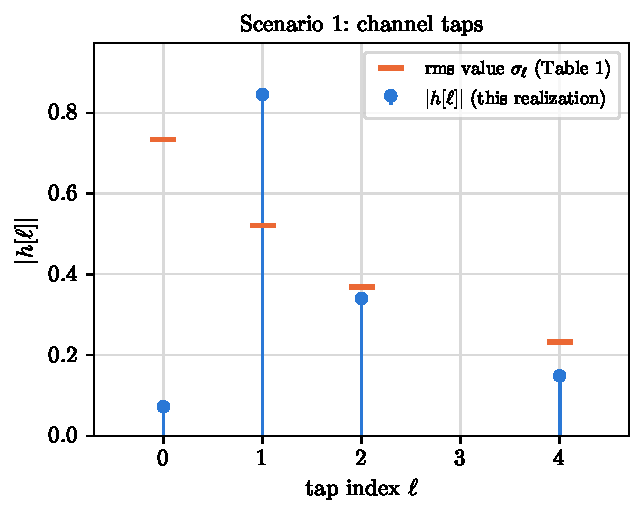
\includegraphics[width=\linewidth]{scenario1_cp4/channel_taps.pdf}
    \caption{Scenario 1, Task 5(a): $|h[\ell]|$ of the realization (stems) and the rms value
      $\sigma_\ell$ of Table 1 (orange).}
    \label{fig:s1-taps}
  \end{minipage}\hfill
  \begin{minipage}[t]{0.485\textwidth}
    \centering
    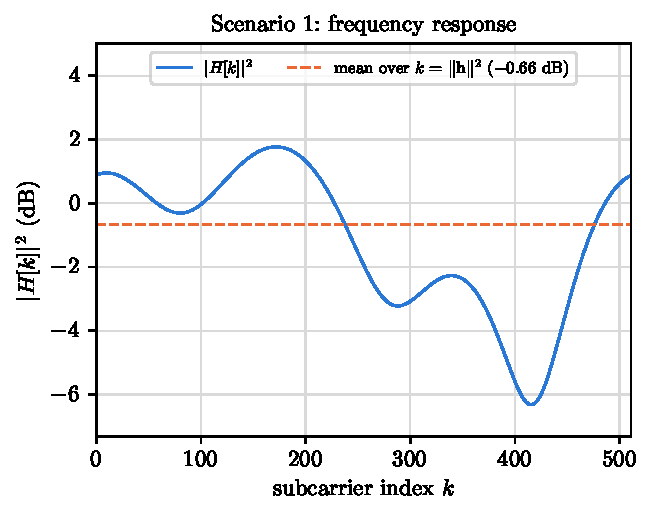
\includegraphics[width=\linewidth]{scenario1_cp4/frequency_response.pdf}
    \caption{Scenario 1, Task 5(a): $|H[k]|^2$ in dB. \textbf{Smooth, from $-6.3$ to $+1.8$ dB.}}
    \label{fig:s1-response}
  \end{minipage}
\end{figure}

\begin{figure}[!htb]
  \centering
  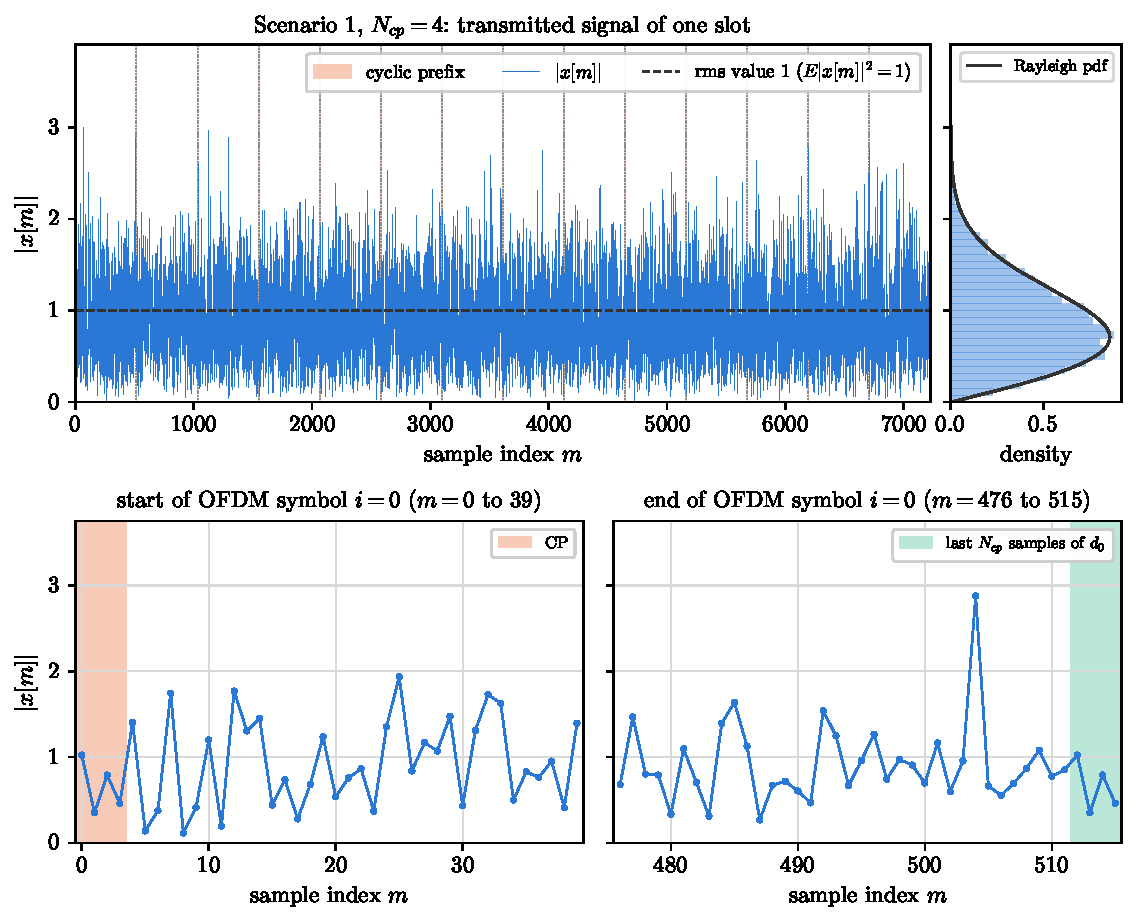
\includegraphics[width=\textwidth]{scenario1_cp4/transmitted_signal.pdf}
  \caption{Scenario 1 ($\Ncp = 4$), Task 5(b): $|x[m]|$ for the $M = 7224$ samples of one slot.
    Dotted lines: start of each OFDM symbol; the 4-sample CPs (orange) are too thin to see at this
    scale. Right: histogram of $|x[m]|$ and the Rayleigh density $2r e^{-r^2}$.
    \textbf{The signal looks like noise with a Rayleigh amplitude; PAPR 9.55 dB.}}
  \label{fig:s1-x}
\end{figure}

\textbf{(a) Channel} (Figs.~\ref{fig:s1-taps} and \ref{fig:s1-response}).
\begin{itemize}
  \item The realization is dominated by tap 1 ($|h[1]|^2 = 0.715$); tap 0 is almost zero.
        $\|h\|^2 = 0.858$ ($-0.66$ dB), which is also the mean of $|H[k]|^2$ over $k$ (Parseval).
  \item $|H[k]|^2$ changes slowly and smoothly, from $-6.3$ dB ($k = 416$) to $+1.8$ dB ($k = 172$).
        No subcarrier is below $-10$ dB.
  \item The reason is the short channel: $H[k]$ is a polynomial of degree 4 in $e^{-j2\pi k/N}$, so it has
        at most 4 dips over the whole band. The coherence bandwidth is about 98 subcarriers.
\end{itemize}

\textbf{(b) Transmitted signal} (Fig.~\ref{fig:s1-x}).
\begin{itemize}
  \item $|x[m]|$ looks like noise. Each $x[m]$ is a sum of 512 independent symbols with different
        phases, so it is close to $\mathcal{CN}(0, 1)$ and $|x[m]|$ is Rayleigh distributed: the
        measured mean is 0.885 against $\sqrt{\pi}/2 = 0.886$.
  \item The average power is 1.0000, but peaks reach about 3 times the rms value:
        the peak-to-average power ratio (PAPR) is 9.55 dB, a known drawback of OFDM.
  \item The 14 OFDM symbols follow each other without gaps; each starts with its 4-sample CP.
\end{itemize}

\begin{figure}[!htb]
  \centering
  \begin{minipage}[t]{0.485\textwidth}
    \centering
    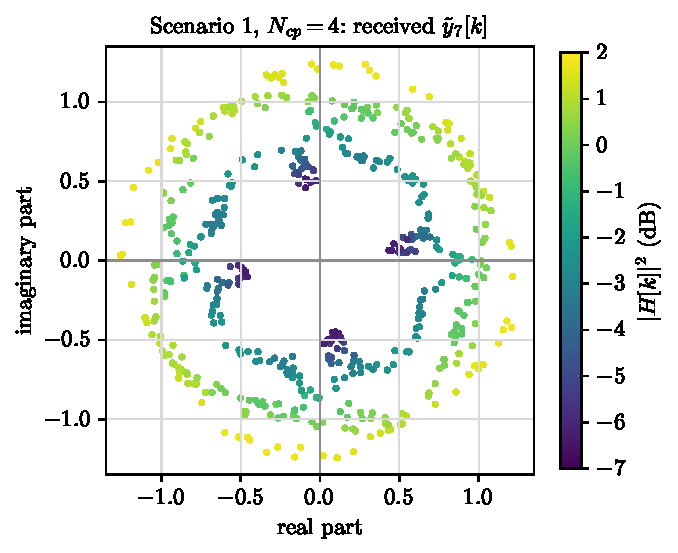
\includegraphics[width=\linewidth]{scenario1_cp4/received_symbols.pdf}
    \caption{Scenario 1 ($\Ncp = 4$), Task 5(c): received values $\yt_7[k]$, before the equalizer.
      \textbf{Four arms: four rotated copies of the curve $H[k]$.}}
    \label{fig:s1-rx}
  \end{minipage}\hfill
  \begin{minipage}[t]{0.485\textwidth}
    \centering
    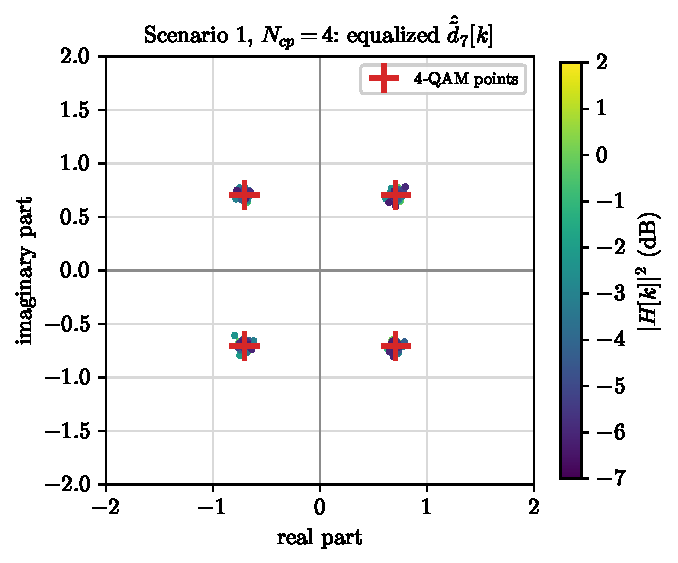
\includegraphics[width=\linewidth]{scenario1_cp4/equalized_symbols.pdf}
    \caption{Scenario 1 ($\Ncp = 4$), Task 5(c): equalized values $\deq_7[k]$ and the 4-QAM points
      (red). \textbf{Four tight clusters; no errors.}}
    \label{fig:s1-eq}
  \end{minipage}
\end{figure}

\begin{figure}[!htb]
  \centering
  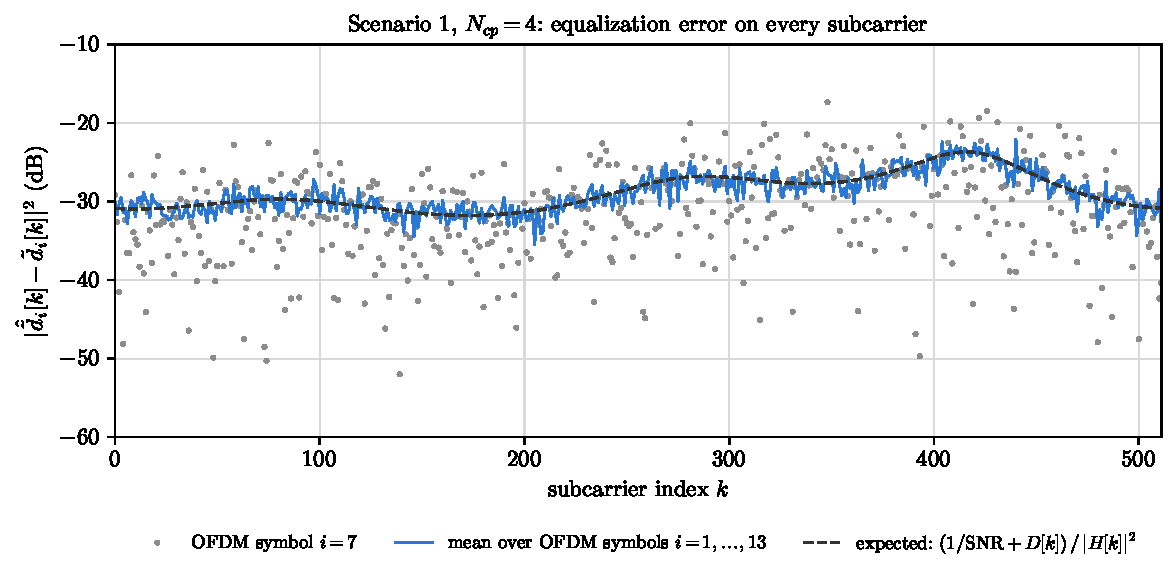
\includegraphics[width=\textwidth]{scenario1_cp4/equalization_error.pdf}
  \caption{Scenario 1 ($\Ncp = 4$), extra figure for Task 5(c): error power after the equalizer on
    every subcarrier. Grey: OFDM symbol 7; blue: mean over the OFDM symbols 1--13; dashed: the
    expected value \eqref{eq:eqnoise} (here $D[k] = 0$). \textbf{The error is the mirror image of
    $|H[k]|^2$ (Fig.~\ref{fig:s1-response}): $-30$ dB $- |H[k]|^2_{\mathrm{dB}}$.}}
  \label{fig:s1-error}
\end{figure}

\textbf{(c) Equalization} (Figs.~\ref{fig:s1-rx}--\ref{fig:s1-error}).
\begin{itemize}
  \item \textbf{Received values.} By \eqref{eq:flat}, each data symbol is rotated by $\angle H[k]$
        and scaled by $|H[k]|$, plus noise. Since $H[k]$ changes smoothly with $k$, the 512 points lie
        on four ``arms'': copies of the curve $H[k]$ in the complex plane, one for each 4-QAM point,
        rotated by $90^\circ$ from each other. The distance from the origin is $|H[k]|$, between 0.48
        (dark) and 1.23 (yellow). A decision is not possible here: the phase of $H[k]$ moves the points
        through all four quadrants.
  \item \textbf{Equalized values.} All 512 points are in four tight clusters around the 4-QAM points.
  \item \textbf{Spread and $|H[k]|^2$.} By \eqref{eq:eqnoise}, the rms error is $1/\sqrt{\SNR |H[k]|^2}$:
        from 0.026 on the strongest subcarrier ($+1.8$ dB) to 0.065 on the weakest ($-6.3$ dB), so the
        darker points spread a little more. The decision boundary is $1/\sqrt{2} = 0.71$ away,
        more than 10 times the largest rms error. $\SNR_k$ is between 23.7 and 31.8 dB.
  \item \textbf{Numbers} (\texttt{scenario1\_cp4/summary.txt}). Fig.~\ref{fig:s1-error} follows
        \eqref{eq:eqnoise}: the mean error over symbols 1--13 is $1.522 \cdot 10^{-3}$, expected
        $1.519 \cdot 10^{-3}$. Before the equalizer, $\yt - H\dt$ has power $1.010 \cdot 10^{-3}$, equal to
        the noise $10^{-3}$, so no ISI or ICI is left. There are 0 symbol errors in the slot
        (expected 0.00 from \eqref{eq:ser}).
\end{itemize}

\FloatBarrier
% ---------------------------------------------------------------------
\subsection{\texorpdfstring{Scenario 2 ($\Ncp = 75$)}{Scenario 2 (Ncp = 75)}}
% ---------------------------------------------------------------------

\begin{figure}[!htb]
  \centering
  \begin{minipage}[t]{0.485\textwidth}
    \centering
    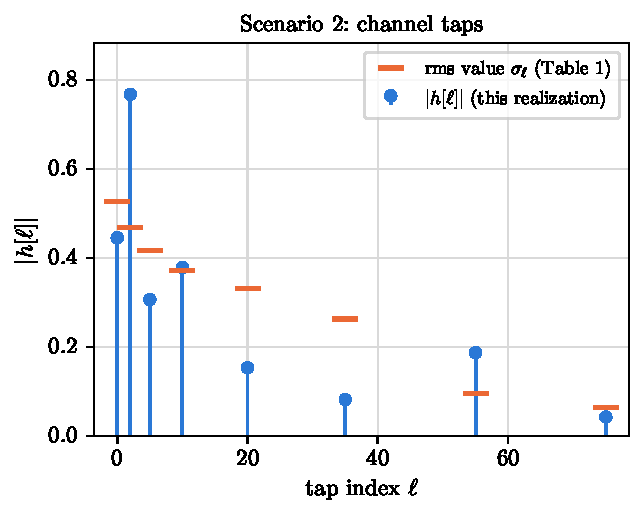
\includegraphics[width=\linewidth]{scenario2_cp75/channel_taps.pdf}
    \caption{Scenario 2, Task 5(a): $|h[\ell]|$ of the realization (stems) and the rms value
      $\sigma_\ell$ of Table 1 (orange).}
    \label{fig:s2-taps}
  \end{minipage}\hfill
  \begin{minipage}[t]{0.485\textwidth}
    \centering
    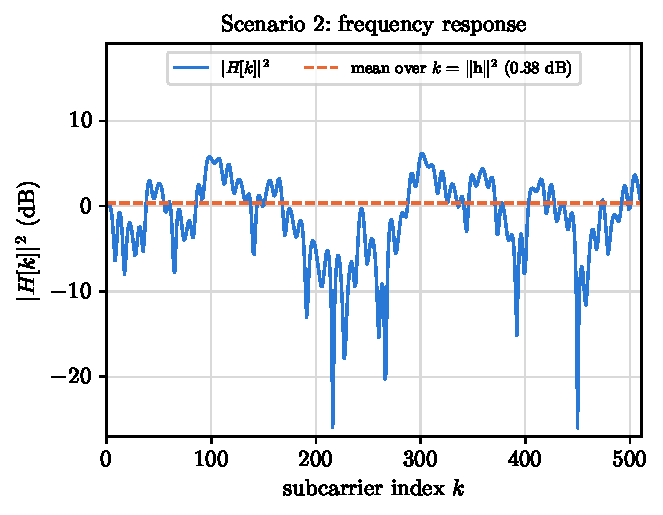
\includegraphics[width=\linewidth]{scenario2_cp75/frequency_response.pdf}
    \caption{Scenario 2, Task 5(a): $|H[k]|^2$ in dB. \textbf{Fast changes and deep fades, from $-26.0$
      to $+6.2$ dB.}}
    \label{fig:s2-response}
  \end{minipage}
\end{figure}

\begin{figure}[!htb]
  \centering
  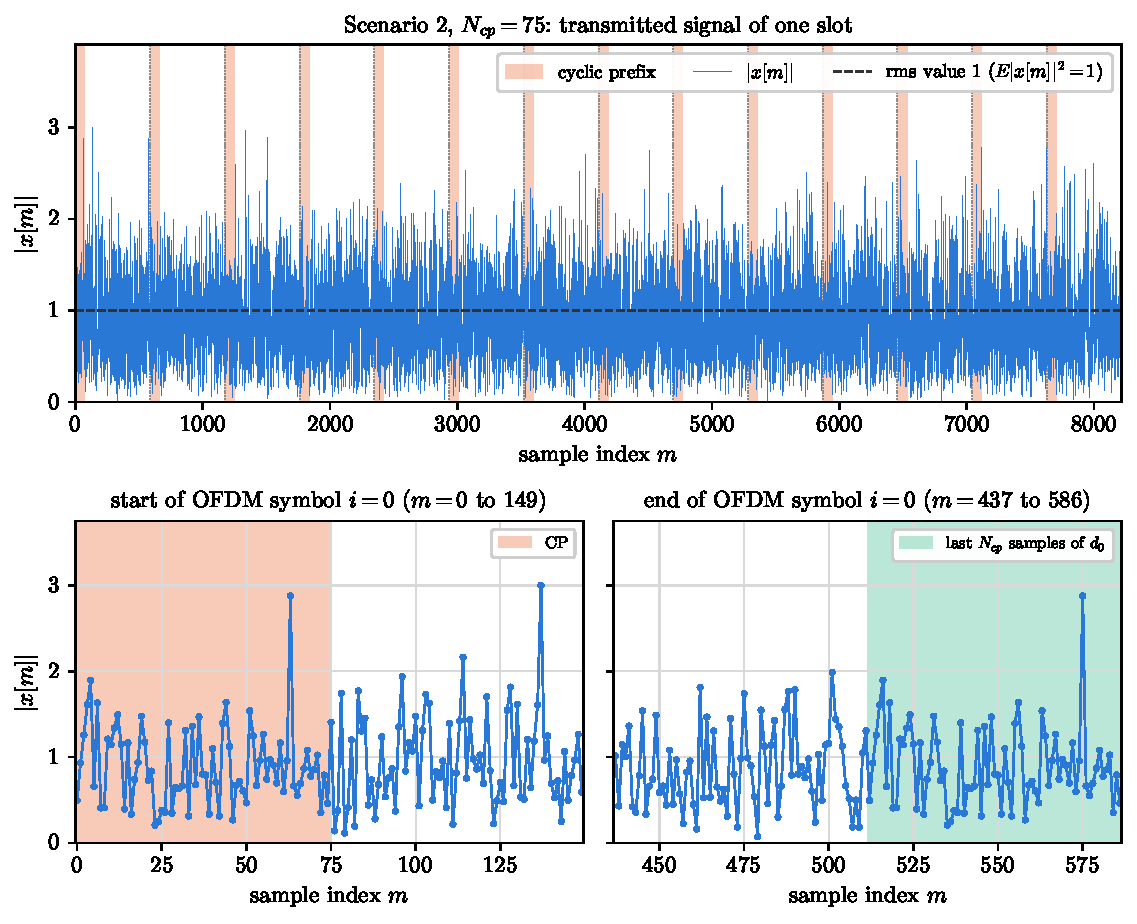
\includegraphics[width=\textwidth]{scenario2_cp75/transmitted_signal.pdf}
  \caption{Scenario 2 ($\Ncp = 75$), Task 5(b): $|x[m]|$ for the $M = 8218$ samples of one slot.
    Orange: the 75-sample CP of each OFDM symbol. Right: histogram of $|x[m]|$ and the Rayleigh
    density. \textbf{Same noise-like signal as in Scenario 1; 12.8\% of the samples are CP.}}
  \label{fig:s2-x}
\end{figure}

\textbf{(a) Channel} (Figs.~\ref{fig:s2-taps} and \ref{fig:s2-response}).
\begin{itemize}
  \item Eight non-zero taps over 76 positions. Tap 2 is the strongest ($|h[2]|^2 = 0.589$);
        $\|h\|^2 = 1.091$ ($+0.38$ dB).
  \item $|H[k]|^2$ changes fast and has deep fades: 27 subcarriers are below $-10$ dB, the deepest are
        $-26.0$ dB ($k = 450$) and $-25.9$ dB ($k = 216$), and the maximum is $+6.2$ dB ($k = 301$).
  \item The coherence bandwidth is about 9 subcarriers, ten times smaller than in Scenario 1, because
        the delay spread is ten times larger. Still, $\Delta f = 30$ kHz is much smaller than
        $B_c \approx 270$ kHz, so every subcarrier sees a flat channel and one complex gain $H[k]$ per
        subcarrier is enough. This is the purpose of OFDM.
\end{itemize}

\textbf{(b) Transmitted signal} (Fig.~\ref{fig:s2-x}). The signal has the same statistics as in
Scenario 1 (mean $|x[m]|$ = 0.883, PAPR 9.57 dB). Now the 14 CPs of 75 samples are clearly visible.
The average power is 0.9946 instead of exactly 1, because the 75 CP samples repeat random samples
(Sec.~3).

\begin{figure}[!htb]
  \centering
  \begin{minipage}[t]{0.485\textwidth}
    \centering
    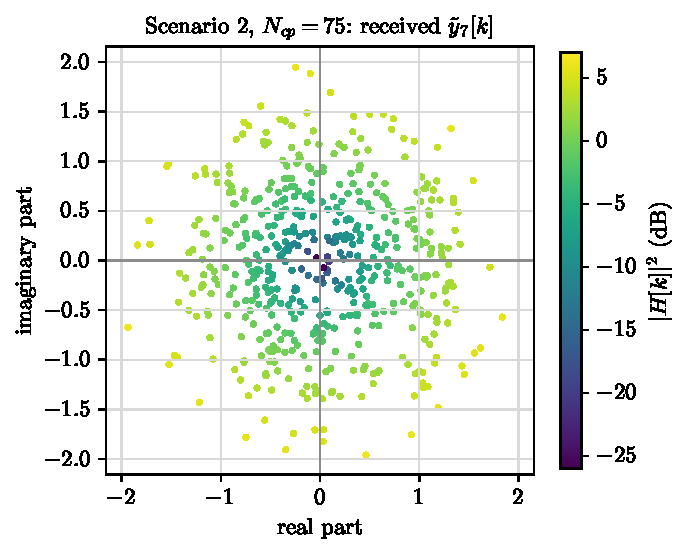
\includegraphics[width=\linewidth]{scenario2_cp75/received_symbols.pdf}
    \caption{Scenario 2 ($\Ncp = 75$), Task 5(c): received values $\yt_7[k]$, before the equalizer.
      \textbf{A cloud without structure; faded subcarriers (dark) near the origin.}}
    \label{fig:s2-rx}
  \end{minipage}\hfill
  \begin{minipage}[t]{0.485\textwidth}
    \centering
    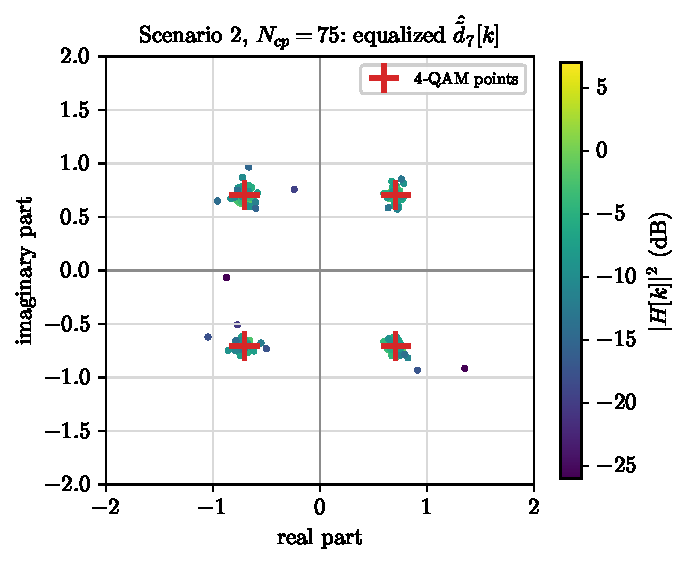
\includegraphics[width=\linewidth]{scenario2_cp75/equalized_symbols.pdf}
    \caption{Scenario 2 ($\Ncp = 75$), Task 5(c): equalized values $\deq_7[k]$ and the 4-QAM points
      (red). \textbf{Tight clusters, except for the faded (dark) subcarriers.}}
    \label{fig:s2-eq}
  \end{minipage}
\end{figure}

\begin{figure}[!htb]
  \centering
  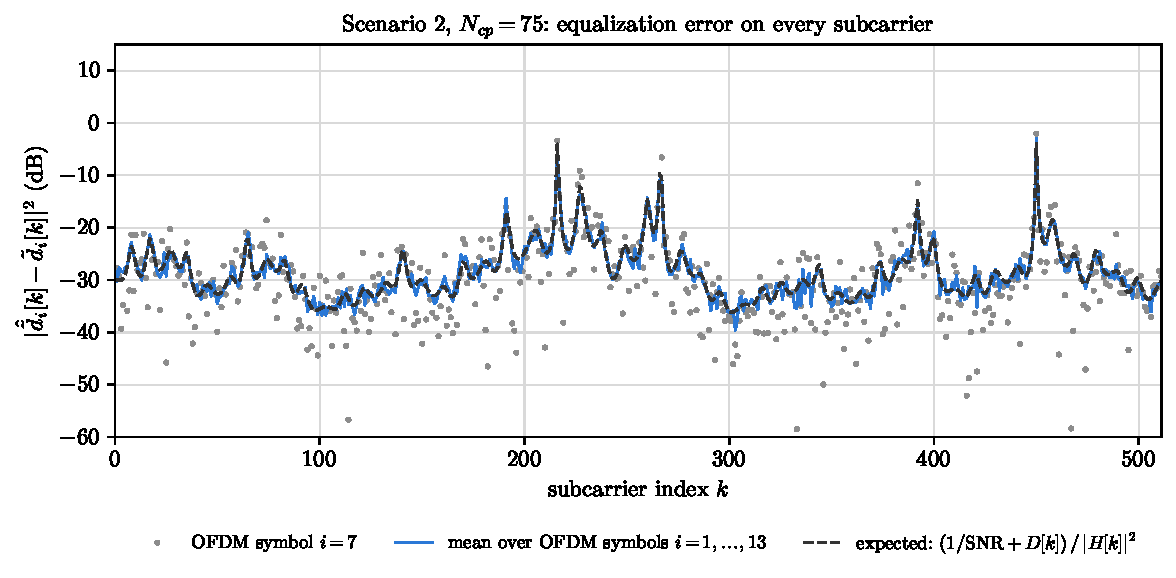
\includegraphics[width=\textwidth]{scenario2_cp75/equalization_error.pdf}
  \caption{Scenario 2 ($\Ncp = 75$), extra figure for Task 5(c): error power after the equalizer on
    every subcarrier, as in Fig.~\ref{fig:s1-error} ($D[k] = 0$). \textbf{The peaks are the fades
    of Fig.~\ref{fig:s2-response}: the noise is multiplied by $1/|H[k]|^2$.}}
  \label{fig:s2-error}
\end{figure}

\textbf{(c) Equalization} (Figs.~\ref{fig:s2-rx}--\ref{fig:s2-error}).
\begin{itemize}
  \item \textbf{Received values.} A round cloud with no visible structure: $H[k]$ changes fast with $k$,
        so neighbouring subcarriers get very different rotations. $|H[k]|$ goes from 0.05 to 2.03; the
        points of the faded subcarriers (dark) are close to the origin.
  \item \textbf{Equalized values.} The strong subcarriers (green, yellow) form tight clusters. The
        faded subcarriers (dark) are spread far from the 4-QAM points.
  \item \textbf{Spread and $|H[k]|^2$.} By \eqref{eq:eqnoise} the rms error is 0.016 on the strongest
        subcarrier ($+6.2$ dB) but 0.63 on the deepest fade ($-26.0$ dB, $k = 450$), close to the
        distance 0.71 to the decision boundary. Dividing by a small $H[k]$ multiplies the noise by
        $1/|H[k]|$ (noise enhancement). $\SNR_k$ goes from 4.0 to 36.2 dB.
  \item \textbf{Numbers} (\texttt{scenario2\_cp75/summary.txt}). On the 226 subcarriers with
        $|H[k]|^2 \ge 0$ dB the mean error is $5.98 \cdot 10^{-4}$ (expected $6.00 \cdot 10^{-4}$); over all
        subcarriers it is $4.57 \cdot 10^{-3}$ (expected $4.70 \cdot 10^{-3}$), dominated by the few deep
        fades. Before the equalizer, $\yt - H\dt$ has power $1.013 \cdot 10^{-3}$: only noise, as in
        Scenario 1. There is 1 symbol error in the slot, in symbol 7 on subcarrier $k = 450$, the deepest
        fade. \eqref{eq:ser} expects 3.1 errors, almost all from the deepest fades; with so few errors,
        1 is a normal result.
\end{itemize}

\FloatBarrier
% ---------------------------------------------------------------------
\subsection{Comparison of the two scenarios}
% ---------------------------------------------------------------------

\begin{table}[!htb]
  \centering
  \caption{Main numbers of both scenarios with the designed CP, from the \texttt{summary.txt} files. ``Expected'' uses \eqref{eq:eqnoise} and \eqref{eq:ser}.}
  \label{tab:compare}
  \small
  \begin{tabular}{lcc}
    \toprule
    & Scenario 1, $\Ncp = 4$ & Scenario 2, $\Ncp = 75$ \\
    \midrule
    CP overhead                                    & 0.78\%                & 12.78\% \\
    $\|h\|^2$                                       & 0.858 ($-0.66$ dB)    & 1.091 ($+0.38$ dB) \\
    $|H[k]|^2$ min / max                           & $-6.3$ / $+1.8$ dB    & $-26.0$ / $+6.2$ dB \\
    Subcarriers with $|H[k]|^2 < -10$ dB           & 0                     & 27 \\
    $\SNR_k = \SNR |H[k]|^2$                       & 23.7 to 31.8 dB       & 4.0 to 36.2 dB \\
    PAPR of $x$                                    & 9.55 dB               & 9.57 dB \\
    Power of $\yt - H\dt$, measured / expected      & $1.010 / 1.000 \cdot 10^{-3}$ & $1.013 / 1.000 \cdot 10^{-3}$ \\
    Mean error after equalizer, measured / expected & $1.52 / 1.52 \cdot 10^{-3}$   & $4.57 / 4.70 \cdot 10^{-3}$ \\
    Symbol errors in the slot (expected)           & 0 (0.00)              & 1 (3.08) \\
    \bottomrule
  \end{tabular}
\end{table}

\begin{itemize}
  \item With the designed CP, both receivers see exactly $\yt = H\dt + \wt$: the disturbance power before
        the equalizer equals the noise power. The CP removes all ISI and ICI in both scenarios.
  \item The scenarios differ only in frequency selectivity. The mean channel power is about the same,
        but Scenario 2 has deep fades, and its only error comes from the deepest one, not from the CP.
        A real system protects these subcarriers with channel coding across the band.
\end{itemize}

\FloatBarrier
% ---------------------------------------------------------------------
\subsection{Task 5(d): insufficient CP}
\label{sec:short}
% ---------------------------------------------------------------------

The slot is sent over the \emph{same} Scenario 2 channel with the same data, but with $\Ncp = 4$.

\begin{figure}[!htb]
  \centering
  \begin{minipage}[t]{0.485\textwidth}
    \centering
    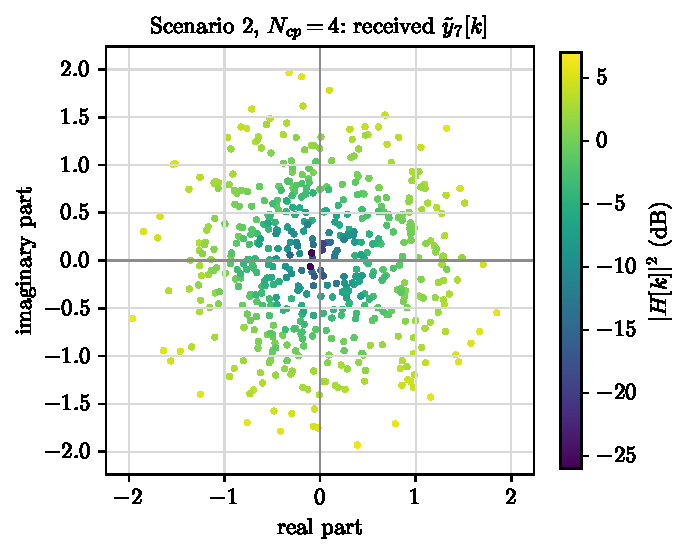
\includegraphics[width=\linewidth]{scenario2_cp4/received_symbols.pdf}
    \caption{Scenario 2 with a too short CP ($\Ncp = 4$), Task 5(d): received values $\yt_7[k]$.
      \textbf{Almost the same as Fig.~\ref{fig:s2-rx}.}}
    \label{fig:short-rx}
  \end{minipage}\hfill
  \begin{minipage}[t]{0.485\textwidth}
    \centering
    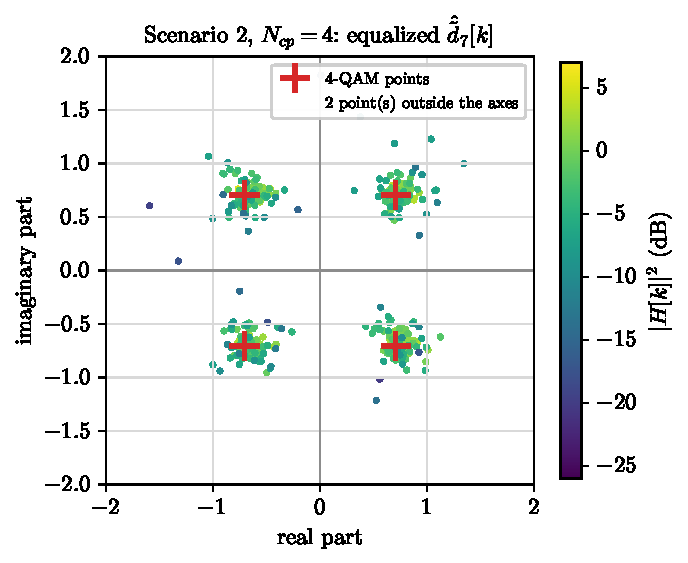
\includegraphics[width=\linewidth]{scenario2_cp4/equalized_symbols.pdf}
    \caption{Scenario 2 with a too short CP ($\Ncp = 4$), Task 5(d): equalized values $\deq_7[k]$.
      \textbf{Wide clusters, also on strong subcarriers.}}
    \label{fig:short-eq}
  \end{minipage}
\end{figure}

\begin{figure}[!htb]
  \centering
  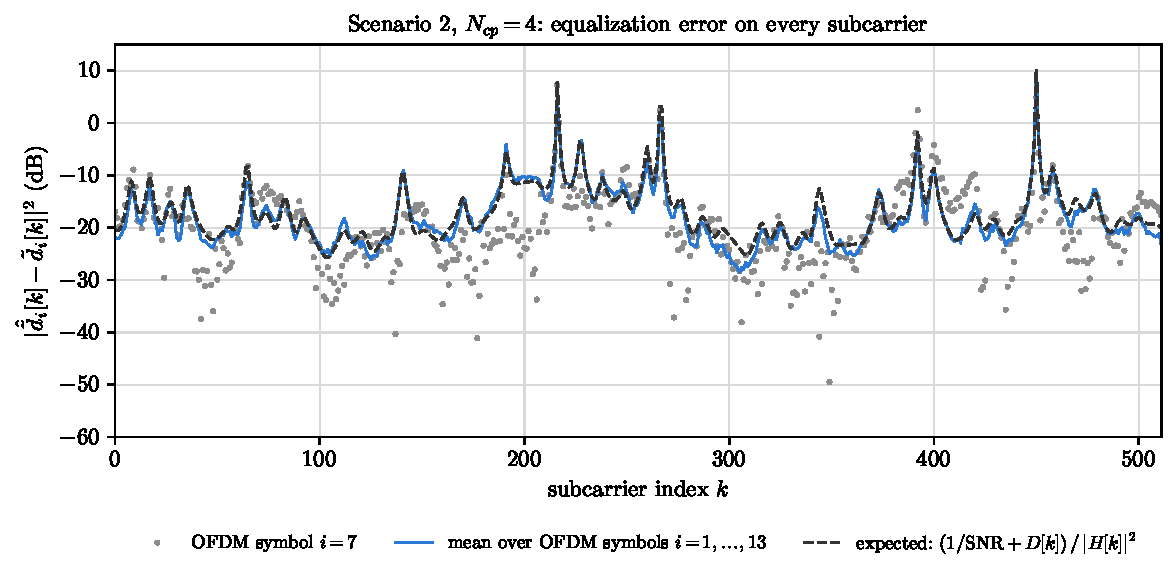
\includegraphics[width=\textwidth]{scenario2_cp4/equalization_error.pdf}
  \caption{Scenario 2 with a too short CP ($\Ncp = 4$), extra figure for Task 5(d): error power after
    the equalizer on every subcarrier. Dashed: $(1/\SNR + D[k])/|H[k]|^2$, with the ISI + ICI power
    $D[k]$ of App.~\ref{app:interference}. Same axes as Fig.~\ref{fig:s2-error}.
    \textbf{On every subcarrier the expected error is 7.9 to 15.0 dB higher than with $\Ncp = 75$ (median 11.2 dB).}}
  \label{fig:short-error}
\end{figure}

\textbf{What goes wrong.} The taps at $\ell = 5, 10, 20, 35, 55, 75$ are longer than the CP. By
\eqref{eq:window}, for the first $\ell - 4$ samples of every DFT window they read the previous OFDM
symbol. This has two effects:
\begin{itemize}
  \item \textbf{ISI:} part of symbol $i-1$ enters the DFT window of symbol $i$.
  \item \textbf{ICI:} the window no longer holds a circular convolution of $d_i$, so \eqref{eq:flat} no
        longer holds. The subcarriers are not orthogonal any more, and every $\yt_i[k]$ also gets parts of
        the other $\dt_i[k']$.
\end{itemize}
Both add an error $\tilde{e}_i[k]$ to \eqref{eq:flat}: $\yt_i[k] = H[k]\dt_i[k] + \tilde{e}_i[k] + \wt_i[k]$. Its power
$D[k]$ is derived in Appendix~\ref{app:interference}. It is not reduced by more transmit power, because
it grows with the signal: it is an error floor.

\begin{table}[!htb]
  \centering
  \caption{ISI + ICI power of each tap beyond the CP, $(2/N)|h[\ell]|^2(\ell - \Ncp)$, for $\Ncp = 4$
    (\texttt{scenario2\_cp4/summary.txt}).}
  \label{tab:tapshare}
  \small
  \begin{tabular}{ccccc}
    \toprule
    Tap $\ell$ & $|h[\ell]|^2$ & Excess delay $\ell - \Ncp$ & Power ($10^{-3}$) & Share \\
    \midrule
     5 & 0.0937 &  1 & 0.37          & 2.7\% \\
    10 & 0.1430 &  6 & 3.35          & 24.9\% \\
    20 & 0.0234 & 16 & 1.46          & 10.9\% \\
    35 & 0.0066 & 31 & 0.81          & 6.0\% \\
    55 & 0.0349 & 51 & \textbf{6.95} & \textbf{51.8\%} \\
    75 & 0.0018 & 71 & 0.50          & 3.7\% \\
    \midrule
    \multicolumn{3}{l}{Total, $\bar{D}$} & 13.44 & 100\% \\
    \bottomrule
  \end{tabular}
\end{table}

\begin{table}[!htb]
  \centering
  \caption{Scenario 2 with the designed and with a too short CP: same data, same channel
    (\texttt{scenario2\_cp75/} and \texttt{scenario2\_cp4/summary.txt}). $^*$The 226 subcarriers with $|H[k]|^2 \ge 0$ dB.}
  \label{tab:short}
  \small
  \begin{tabular}{lcc}
    \toprule
    & $\Ncp = 75$ (Task 5c) & $\Ncp = 4$ (Task 5d) \\
    \midrule
    ISI + ICI power $\bar{D}$ (mean of $D[k]$)        & 0                                  & $1.344 \cdot 10^{-2}$ ($-18.7$ dB) \\
    Power of $\yt - H\dt$, measured                   & $1.013 \cdot 10^{-3}$ ($-29.9$ dB)  & $1.275 \cdot 10^{-2}$ ($-18.9$ dB) \\
    Power of $\yt - H\dt$, expected                 & $1.000 \cdot 10^{-3}$ ($-30.0$ dB)  & $1.444 \cdot 10^{-2}$ ($-18.4$ dB) \\
    Mean SINR, $\|h\|^2 / (1/\SNR + \bar{D})$         & 30.4 dB                            & 18.8 dB \\
    SINR per subcarrier                              & 4.0 to 36.2 dB                     & $-10.3$ to 25.7 dB \\
    Mean error after equalizer, strong subcarriers$^*$ & $5.98 \cdot 10^{-4}$       & $7.61 \cdot 10^{-3}$ \\
    Symbol errors in OFDM symbol 7                   & 1                                  & 4 \\
    Symbol errors in the slot (expected)             & 1 (3.1)                            & 39 (50.7) \\
    \bottomrule
  \end{tabular}
\end{table}

\textbf{Numbers} (Tables~\ref{tab:tapshare} and \ref{tab:short}).
\begin{itemize}
  \item The ISI + ICI power is $\bar{D} = 1.34 \cdot 10^{-2}$ ($-18.7$ dB), 13 times (11.3 dB) the
        noise power. The mean SINR drops from 30.4 dB to 18.8 dB, a loss of 11.6 dB.
  \item Each tap counts with its excess delay $\ell - \Ncp$. Tap 55 has only 3\% of the channel energy,
        but it reaches 51 samples into the previous symbol and causes half of the interference.
  \item The measured disturbance, $1.275 \cdot 10^{-2}$, is 12\% below the expected
        $1.444 \cdot 10^{-2}$. This is the random variation of one slot: \texttt{cp\_sweep.py} sends 200
        noise-free slots with different random data, and their mean ISI + ICI power is within 0.23\% of
        $\bar{D}$ (on each subcarrier: measured$/D[k] = 0.998 \pm 0.022$), while one slot varies by 7.2\%.
  \item The symbol errors rise from 1 to 39 (4 in symbol 7). They are on 10 subcarriers, all in the
        deepest fades ($-11.8$ to $-26.0$ dB) and next to them, where the SINR is lowest. The expected
        50.7 treats the ISI + ICI as Gaussian noise, which is only an approximation.
\end{itemize}

\textbf{Comparison with plot (c) for Scenario 2.}
\begin{itemize}
  \item \textbf{Before the equalizer} (Fig.~\ref{fig:short-rx} against Fig.~\ref{fig:s2-rx}) the two plots
        look almost the same. The extra disturbance ($-18.9$ dB) is small next to $|\yt| \approx |H| \approx 1$,
        and the cloud is already spread by the channel.
  \item \textbf{After the equalizer} (Fig.~\ref{fig:short-eq} against Fig.~\ref{fig:s2-eq}) the
        difference is clear. With $\Ncp = 75$ only the faded subcarriers were spread. With $\Ncp = 4$
        every cluster is wide, also on strong subcarriers (green and yellow points): on the 226 subcarriers
        with $|H[k]|^2 \ge 0$ dB the mean error is 12.7 times (11.0 dB) larger.
  \item \textbf{Why.} The spread is no longer set by the noise alone. The error after the equalizer is
        $(1/\SNR + D[k])/|H[k]|^2$, and $D[k]$ is about 13 times the noise. Fig.~\ref{fig:short-error}
        shows this: the error follows the new dashed line, 7.9 to 15.0 dB above Fig.~\ref{fig:s2-error}
        (median 11.2 dB), because $D[k]$ itself varies from $-22.8$ to $-15.2$ dB over the subcarriers.
        Even the best subcarrier is limited to an SINR of 25.7 dB, against 36.2 dB with the correct CP.
\end{itemize}

\subsubsection*{Extra: every CP length from 0 to 80}
\label{sec:sweep}

Fig.~\ref{fig:sweep} checks the CP design of Task 1 by simulation: \texttt{cp\_sweep.py} sends the same
slot with every $\Ncp$ from 0 to 80 (same data, channels and noise seed).

\begin{figure}[!htb]
  \centering
  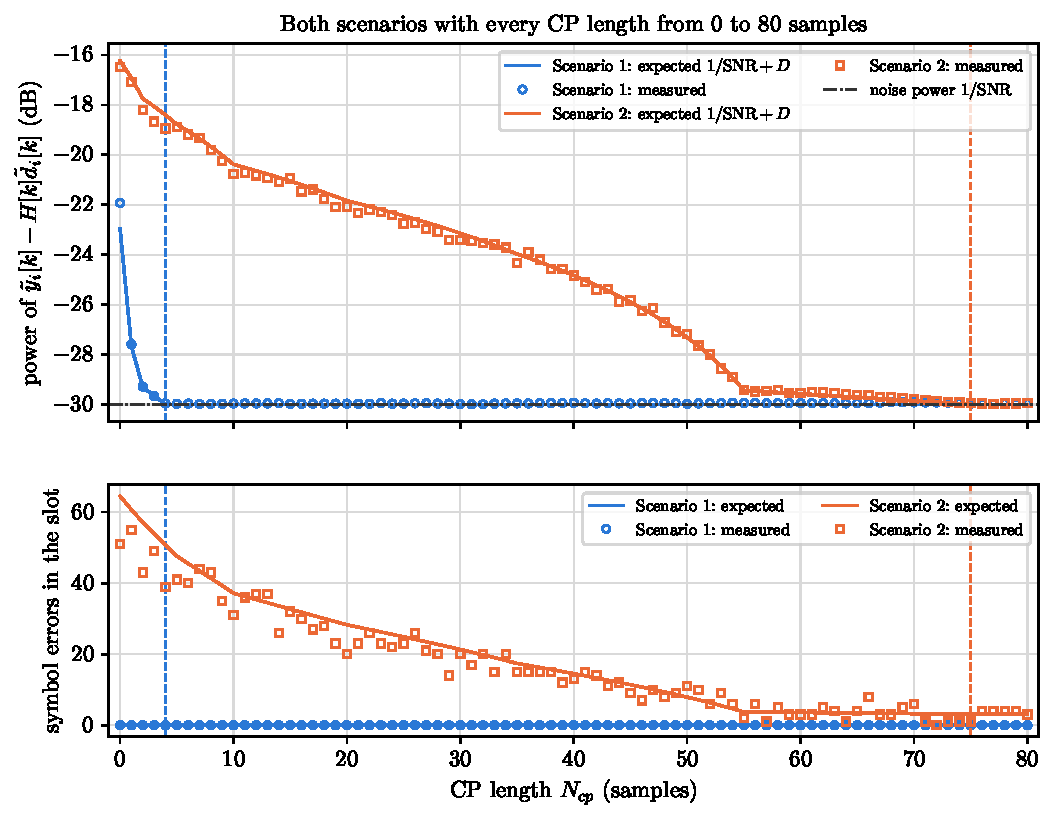
\includegraphics[width=0.85\textwidth]{cp_sweep/cp_sweep.pdf}
  \caption{Both scenarios with every CP length from 0 to 80 samples. Top: power of $\yt_i[k] - H[k]\dt_i[k]$
    (noise + ISI + ICI) over the OFDM symbols 1--13, measured (markers) and expected $1/\SNR + \bar{D}$
    (lines). Bottom: symbol errors in the slot, measured and expected from \eqref{eq:ser}. Dashed
    vertical lines: designed $\Ncp = 4$ (Scenario 1) and 75 (Scenario 2); $\Ncp = 4$ is also the CP of
    Task 5(d). \textbf{The interference ends exactly at $\Ncp = L - 1$; beyond that a longer CP changes
    nothing.}}
  \label{fig:sweep}
\end{figure}

\begin{table}[!htb]
  \centering
  \caption{Scenario 2: selected points of Fig.~\ref{fig:sweep} (\texttt{cp\_sweep/summary.txt}).}
  \label{tab:sweep}
  \small
  \begin{tabular}{ccccc}
    \toprule
    & \multicolumn{2}{c}{Power of $\yt - H\dt$ (dB)} & \multicolumn{2}{c}{Symbol errors in the slot} \\
    \cmidrule(lr){2-3} \cmidrule(lr){4-5}
    $\Ncp$ & measured & expected & measured & expected \\
    \midrule
     0 & $-16.5$ & $-16.2$ & 51 & 64.5 \\
     4 & $-18.9$ & $-18.4$ & 39 & 50.7 \\
    10 & $-20.8$ & $-20.4$ & 31 & 37.2 \\
    20 & $-22.1$ & $-21.8$ & 20 & 28.3 \\
    36 & $-23.9$ & $-24.1$ & 15 & 16.8 \\
    55 & $-29.4$ & $-29.4$ &  2 & 3.8 \\
    74 & $-29.9$ & $-30.0$ &  1 & 3.1 \\
    75 & $-29.9$ & $-30.0$ &  1 & 3.1 \\
    \bottomrule
  \end{tabular}
\end{table}

\begin{itemize}
  \item \textbf{Scenario 1}: the interference is gone at $\Ncp = 4$. From there on the disturbance is
        the noise ($-30.0$ dB) for every longer CP, and there are no errors.
  \item \textbf{Scenario 2}: the interference falls step by step as $\Ncp$ passes the tap delays and reaches
        the noise level exactly at $\Ncp = 75$. The steep drop between 35 and 55 is the strong tap 55 of this
        realization. With the NR-like CP of 36 samples there are still 15 errors instead of 1.
  \item The measured power follows the expected curve at every $\Ncp$, which confirms the formula of
        Appendix~\ref{app:interference}. The expected error counts use the Gaussian approximation; the
        measured counts are 10--30\% lower for short CPs but follow the same trend.
\end{itemize}

\FloatBarrier
% =====================================================================
\section{Summary}
% =====================================================================

\begin{itemize}
  \item \textbf{CP design (Task 1):} $\Ncp = L - 1$, the delay of the last tap. Scenario 1: 4 samples =
        0.260 $\mu$s, overhead 0.78\%. Scenario 2: 75 samples = 4.883 $\mu$s, overhead 12.78\%.
  \item \textbf{Link (Tasks 2--4):} every block is a separate function and was checked on its own. Without
        noise the receiver gets the data back to $10^{-15}$ with the designed CP, and not with a CP one
        sample shorter.
  \item \textbf{Results (Task 5a--c):} with the designed CP each subcarrier is a flat channel,
        $\yt = H\dt + \wt$. After the equalizer the error on subcarrier $k$ has variance
        $1/(\SNR|H[k]|^2)$, so the spread grows on faded subcarriers. Scenario 1 (smooth channel,
        $-6.3$ to $+1.8$ dB) has no errors; Scenario 2 (deep fades down to $-26$ dB) has 1 error, on the
        deepest fade.
  \item \textbf{Too short CP (Task 5d):} with $\Ncp = 4$ in Scenario 2, ISI and ICI add an error 13 times
        the noise power. The clusters widen on every subcarrier, the mean SINR falls by 11.6 dB, and the
        symbol errors rise from 1 to 39.
\end{itemize}

\appendix
% =====================================================================
\section{ISI + ICI power of a too short CP}
\label{app:interference}
% =====================================================================

Let $\Ncp < L - 1$ and $i \ge 1$. In \eqref{eq:window}, tap $\ell$ at window position $m$ reads block $i$
if $m - \ell \ge -\Ncp$ and block $i-1$ otherwise. Write the window as the ideal circular convolution plus
an error:
\begin{gather}
  y_{c,i}[m] = \sum_\ell h[\ell]\, d_i[(m-\ell) \bmod N] + e_i[m] + w_{c,i}[m], \notag \\
  e_i[m] = \sum_{\ell} h[\ell]\, \mathbf{1}\{m - \ell < -\Ncp\}\, \delta_i[m - \ell],
\end{gather}
where, for $n = -(L-1), \ldots, -\Ncp - 1$, $\delta_i[n]$ is the sample of symbol $i-1$ that arrives
minus the sample $d_i[n \bmod N]$ that a long CP would deliver. All samples of $d_i$ and $d_{i-1}$ are
uncorrelated with unit power (because $F$ is unitary), so the $\delta_i[n]$ are uncorrelated with
$\E|\delta_i[n]|^2 = 2$. Taking the DFT and setting $q = -n$:
\begin{equation}
  \tilde{e}_i[k] = \frac{1}{\sqrt{N}} \sum_{q = \Ncp + 1}^{L-1} \delta_i[-q]\, e^{j2\pi kq/N}\, H_q[k], \qquad
  H_q[k] = \sum_{\ell \ge q} h[\ell]\, e^{-j2\pi k\ell/N},
\end{equation}
where $H_q$ is the response of only those taps that reach $q$ or more samples back. Hence
\begin{equation}
  D[k] = \E|\tilde{e}_i[k]|^2 = \frac{2}{N} \sum_{q = \Ncp + 1}^{L-1} |H_q[k]|^2 .
  \label{eq:dk}
\end{equation}
Averaging over $k$ with Parseval, $\frac{1}{N}\sum_k |H_q[k]|^2 = \sum_{\ell \ge q} |h[\ell]|^2$, gives
\begin{equation}
  \bar{D} = \frac{2}{N} \sum_{q = \Ncp+1}^{L-1} \sum_{\ell \ge q} |h[\ell]|^2
          = \frac{2}{N} \sum_\ell |h[\ell]|^2 \max(\ell - \Ncp, 0),
\end{equation}
and averaging over the channel ($\E|h[\ell]|^2 = \sigma_\ell^2$) gives \eqref{eq:pint}.
\begin{itemize}
  \item The error holds both effects: the part from $d_{i-1}$ is ISI, and the part from $d_i$ mixes
        the subcarriers of symbol $i$ (ICI).
  \item Symbol 0 has nothing before it ($x[m] = 0$ for $m < 0$), so $\E|\delta_0[n]|^2 = 1$ and it sees half
        of $D[k]$. This is why the averages in Task 5 use the OFDM symbols 1--13.
  \item After the equalizer the error power is $(1/\SNR + D[k])/|H[k]|^2$ (dashed line in
        Fig.~\ref{fig:short-error}), and treating $\tilde{e}_i$ as Gaussian, $\SNR_k$ in \eqref{eq:ser} becomes the
        SINR $|H[k]|^2 / (1/\SNR + D[k])$.
\end{itemize}
\texttt{interference\_power\_per\_subcarrier} in \texttt{Task-1/cp\_design.py} computes \eqref{eq:dk}
with one FFT per $q$. The check in Sec.~\ref{sec:short} confirms it: over 200 noise-free slots of random
data, the measured ISI + ICI power is within 0.23\% of $\bar{D}$.

\end{document}
